\chapter{Embedded ML Infrastructure for Plasma Characterization}

\section{A new “smart” DAQ chain proposal for features extraction ( lavoro con Marco Gottardo )}

% smart sensory
% feature extraction concept

In order to collect magnetic field measurements from EM probes, analog integration system~\cite{pomaro2005transducers} was implemented in RFX-mod, followed by two separate sets of ADC channels, one for precision off-line transient data and the other for real-time control. Re-implementing the same front-end for an increased number of channels is costly, requiring enhanced analog integration and duplication in ADC channels.  A more compact and cost effective solution is being investigated~\cite{gottardo18}, using a configurable FPGA to handle ADC conversion and providing a set of on-line functions directly performed at the FPGA logic level, including the numeric integration in real-time, recording at the same time the dB/dt signals deriving directly from EM coils needed to study the Magneto Hydro Dynamic (MHD) processes taking place into the plasma~\cite{zuin2009current}~\cite{innocente2014tearing}. The possibility of directly acquiring the time derivative of the electromagnetic fields, i.e. the direct signals from EM probes, was not present in the previous system, acquiring integrated signals in order to reduce the number of required ADC channels. This fact introduced a severe limitation in the derivative control required for MHD stabilization because of the bad quality of the computed time derivative.

The proposed approach will further reduce the number of ADC channels by merging high frequency transient recording in local memory (up to 1 MHz) and lower frequency streaming (up to 10 kHz) required for real-time plasma control and having a single ADC channel performing both. In RFX-mod a fixed subset of signals from EM probes was used for the active plasma control, requiring a new set of ADC converters in respect to the transient recorders used for data acquisition. In RFX-mod2 it will be possible to re-use any ADC channel from EM probes for real-time plasma control, being the actual number possibly limited by other factors not related to the ADC devices, such as network bandwidth or control computation load. 
%
The flexibility provided by a configurable on board FPGA allows also the inclusion of more sophisticated triggering mechanisms and a deeper integration with the timing systems. Examples of triggering mechanism are given by the acquisition of fast transients requiring high speed sampling only in a given, dynamic Region of Interest (ROI). This feature has been implemented in the first proof-of-concept device described in a later section. Deeper integration with the timing systems imply the ability of getting the clock and the trigger signals not only from digital inputs, but also from the specifically coded signal carrying both clock and trigger information (timing highway)\cite{dio4}. Such signals were used in the RFX-mod timing systems to distribute a synchronous clock and asynchronous triggers and a timing device was required for every ADC rack to extract the clock and the trigger signals. The timing device is no more required for a rack hosting the new ADC devices because the ADC devices can directly extract timing information from the timing highway.  
%
The adoption of a System on Chip (SoC) based technology exploiting both an ARM based processing unit and a FPGA logic provides the  flexibility of a configurable device for real-time operations and as well as the possibility of deploying software components directly on-board. The Red Pitaya board~\cite{redpitaya} is currently used for the development of the architecture. A different solution is however foreseen for the production system integrating an external ADC section with the Zynq-based SoC board. An ADC front end, already used in other applications of real-time plasma control~\cite{ATCA-MIMO-ISOL} was initially considered, but its noise characteristics, and in particular the noise dependency on frequency, proved to limit the quality of digital integration. For this reason, a different solution for the ADC stage is being considered.

The first implementation of the flexible ADC architecture has been carried out on a Red Pitaya board, using the in-board ADC channels. Even if not intended to represent the final application, development of FPGA logic on Red Pitaya offers the advantage of a ready-to-use ADC channel for development and first tests. Most of the firmware will be retained in the final implementation, using a different ADC front end. 
%
The time critical functions carried out by the FPGA in this context are:
\begin{itemize}
\item The management of a circular data buffer and the DMA transfer in RAM of pre and post trigger samples after the trigger has been received;
\item anti-aliasing filtering and subsequent sub-sampling of the samples to be streamed. The resulting samples are enqueued in a FIFO accessed by the processor;
\item digital integration for deriving magnetic field measurements from EM probe signals. Observe that in this case a single ADC stage will generate two ADC channels;
\item ROI detection in case ADC triggers are derived from the signal itself (e.g. over a given signal level threshold);
\item Clock and trigger extraction in case a highway signal is provided by the timing system, encoding both clock an triggers.
\end{itemize}
%
The less critical functions that will be carried out by the processor unit are:
\begin{itemize}
\item The management of the configuration setting, received via TCP/IP or HTTP. The processor validates the configuration and write the appreciate registers in the FPGA;
\item off-line data readout of acquired samples in transient recording and communication via TCP/IP with the central data acquisition system;
\item network data streaming of sub-sampled data read from the FIFO and sent in UDP packets to the active plasma control system. 
\end{itemize}
%
In addition to pre-configured blocks from the XILINX toolbox for data buffering, DMA engine, I/O FIFO and registers, three blocks implemented in VHDL carry out the underlying logic. The first block provides the management of clock and triggers that may be either directly derived from digital inputs or rebuild by properly decoding the timing highway input signal. The second block provides programmable input signal elaboration such as low pass filtering for subsampling and integration. The third block will handle the triggering logic and the circular buffer holding pre and post trigger samples. In particular, the trigger may be derived from external signals (via the first block) or derived from the input signal (e.g. when the input level is greater than a given threshold).    

Communication of subsamples streamed data for real-time plasma control is achieved using the XILINX AXI Stream FIFO. The Xilinx AXI Stream FIFO is a Xilinx free software IP that implement a read/write FIFO queue with a well defined communication protocol. A proper connected IRQ line is used to trigger events to the processing unit together with the related set of status and enable registers. In this way data samples are readily available to the linux processor and will be sent using low latency UDP communication to computing nodes carrying out distributed for real-time plasma control. Communication of the data acquired at high speed in the ROI is carried out by a DMA engine, using circular DMA buffers in order to minimize the number of data copies. In this case data will be sent to the central Data Acquisition system via TCP/IP as soon as a ROI has been acquired. Fig. 1 shows the main blocks of the ADC device: the external ADC circuitry, communicating with the FPGA via a serial LVDS link; the FPGA logic, communicating with the processor via registers, FIFO and DMA; the processor components, in kernel and user space. 
~
~
\begin{figure}[ht]
\centering
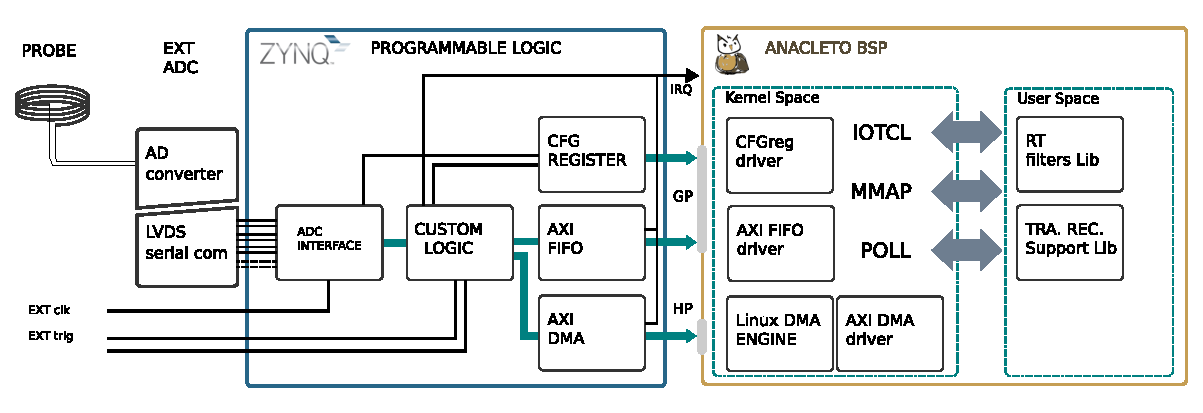
\includegraphics[width=0.9\textwidth]{img/4_EmbeddedML/schema_logico.pdf}
\caption{Logic design of the flexible ADC structure.}
\label{fig:logic}
\end{figure}





%%
%% NIO ADC % ANDREA
%%
\section{A proof-of-concept implementation: fast streamed event driven data acquisition for the NIO negative ion beam}
~
Another desired topics for a DAQ device is the possibility to increase the level of detail during acquisition based on particular events. It is not uncommon to have an observed quantity that changes rapidly in time and than last steady or possibly in a non interesting state for long periods. An example of is the breakdown event that occurs in the accelerator grids of a ion source, leading to a very fast transient change in the measured currents and voltages of the grid power supply. In this case, fast data acquisition must be triggered by the event itself, acquiring data for a short time window around the event occurrence. This technique has been applied to Nio experiment~\cite{DEMURI2015249} a small radio frequency negative ions beam source with a high voltage electrostatic particle accelerator stage composed of grids. In certain conditions break-down events~\cite{RECCHIA20111545} appear on the high voltage gaps of the grids causing a  high current discharges of the power supply feeding the accelerator. 
~
A subset of the FPGA functionality described in section 3 has been implemented in a Red Pitaya device, namely the trigger logic to detect the occurrence of the event, the pre and post trigger sampling logic and the FIFO/DMA data transfer to computer memory via the GNU Linux driver. In this case data are streamed and when an event is detected and data collected at 5 MHz sampling speed along the corresponding time window, the data block is passed, either via FIFO or DMA, to the linux driver and then, in turn, to a program in the Zynq processor that communicates the newly acquired data block to the central data acquisition system via TCP/IP. The results are displayed in Fig. 4, showing the events acquired during a beam generation lasting 2 hours. Each time window lasts 1 ms, and one enlarged event is  displayed in the lower part of Fig. 4.    

\begin{figure}[ht]
\centering
%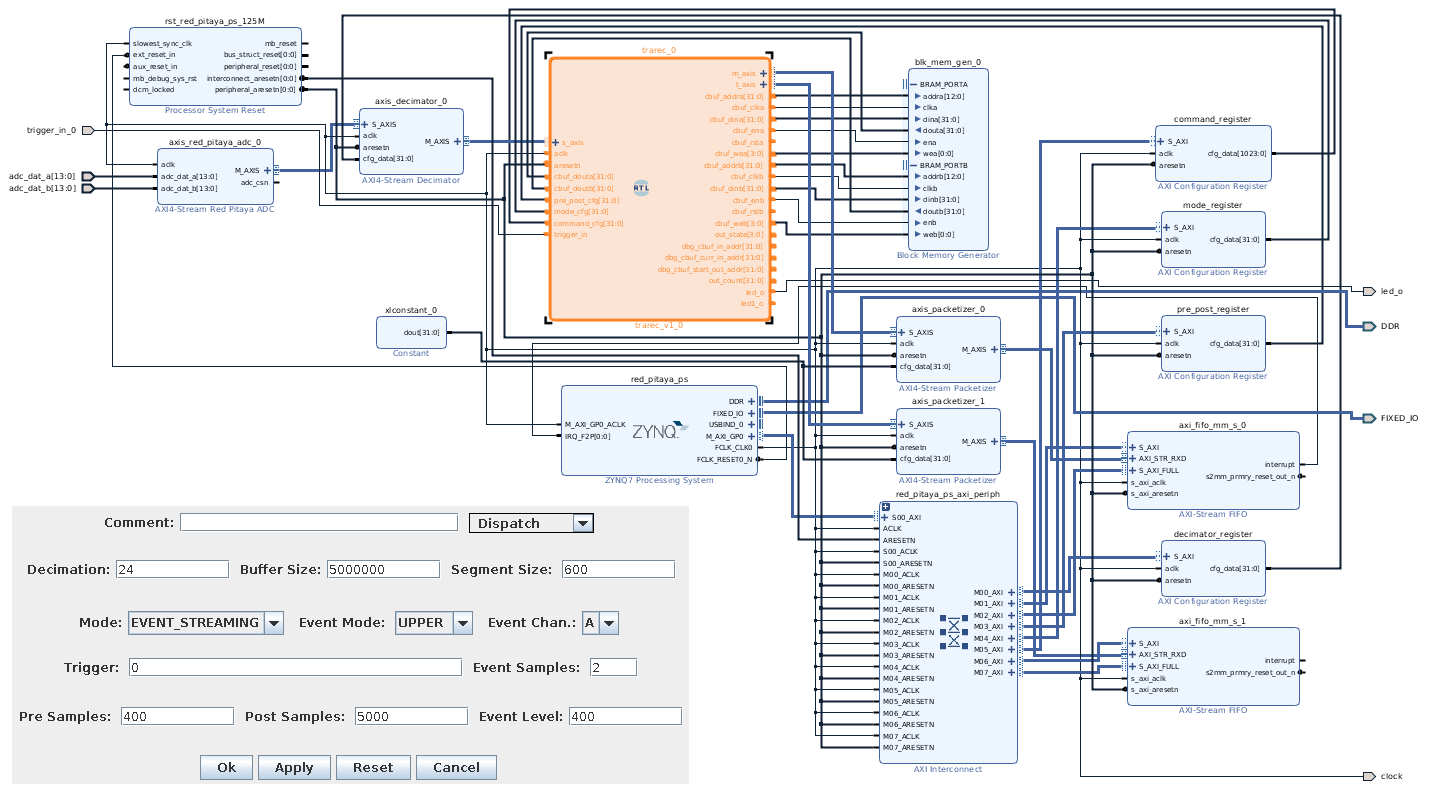
\includegraphics[width=0.59\textwidth]{img/nio_scm1.png}
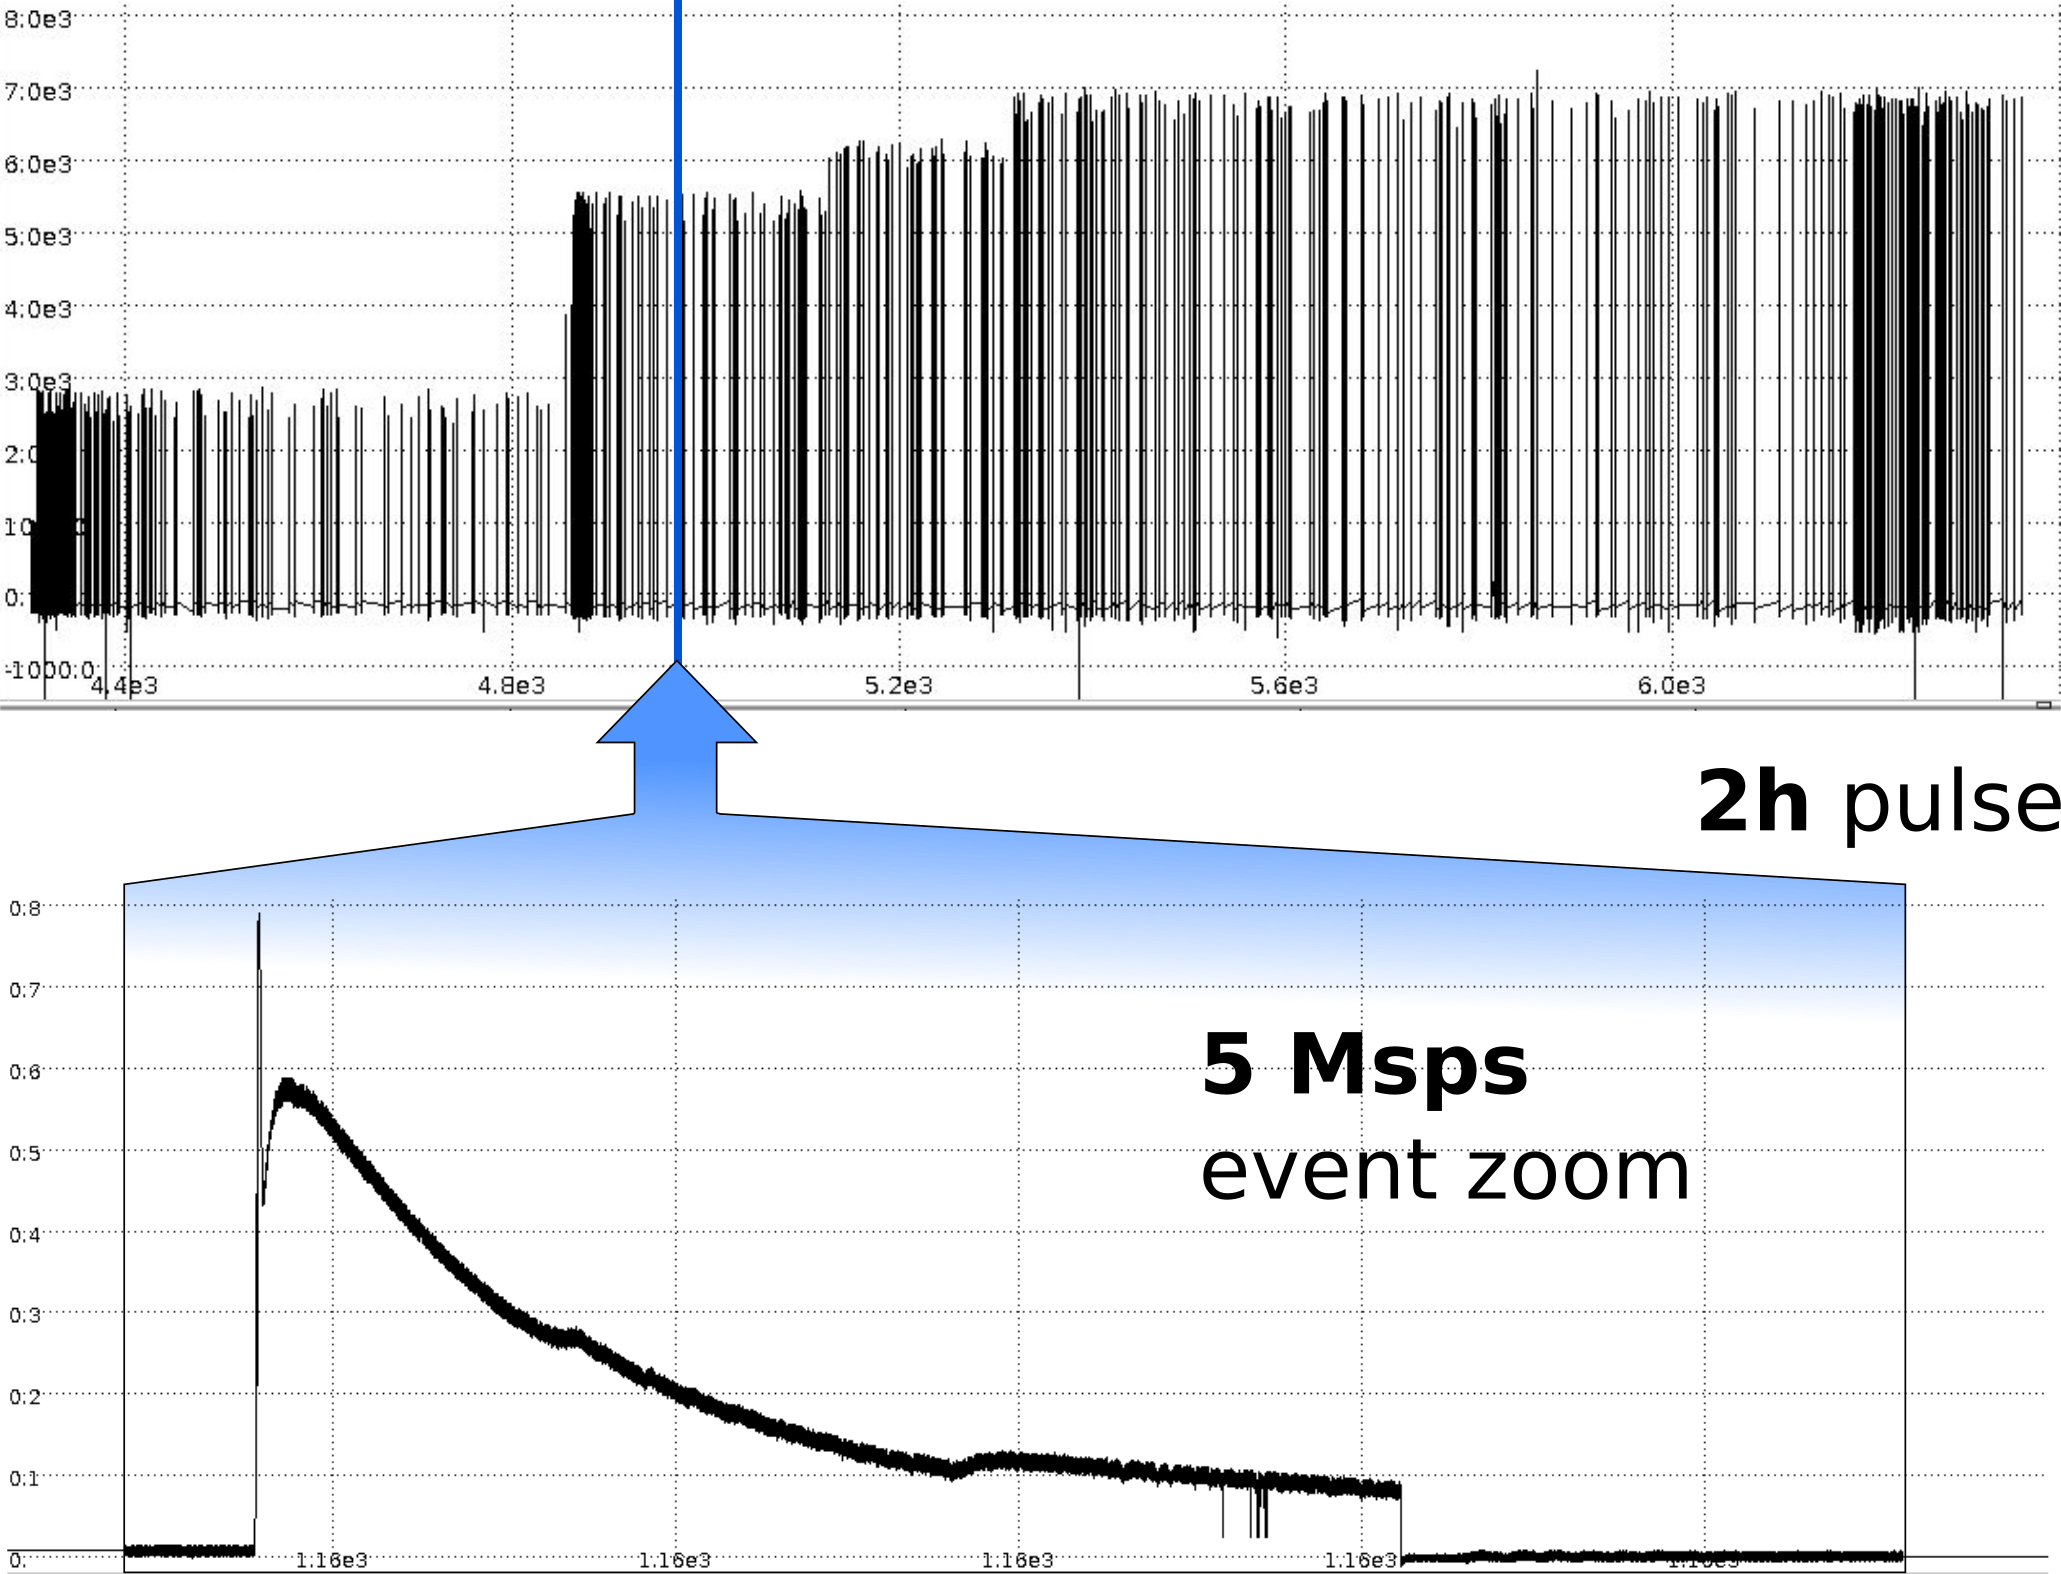
\includegraphics[width=0.49\textwidth]{img/4_EmbeddedML/nio12b.png}
\caption{figure example.}
\label{fig:nio}
\end{figure}




\section{Easing the curse of dimensionality by means of latent space compression}

\section{Quantized neural networks for embedded implementation}
